% 21/08/2018 - v.0.01 - first part of the material
\documentclass[a4paper,11pt]{article}
\usepackage{fullpage}
\usepackage{graphicx}
\usepackage{authblk}
\usepackage{hyperref}

% diagrams
\usepackage{tikz}
%\usepackage{hyperref}
\usetikzlibrary{shapes,arrows}


%%%%%%%%%%%%%%%%%%%%%%%%%%%%%%%%%%%%%%%%%%%%%%%%%%%%%%%%%%%%%%%%%%%%%%%%%%%%%%%%
% used only during the manuscript preparation
%%%%%%%%%%%%%%%%%%%%%%%%%%%%%%%%%%%%%%%%%%%%%%%%%%%%%%%%%%%%%%%%%%%%%%%%%%%%%%%%
\newcommand{\note}[1]{%
    \par\vspace{6pt}\noindent\underline{\textsc{Note:}} \emph{#1}\vspace{6pt}%
}
\newcommand{\todo}[1]{%
    \par\vspace{6pt}\noindent\underline{\textsc{TODO:}} \emph{#1}\vspace{6pt}%
}
%%%%%%%%%%%%%%%%%%%%%%%%%%%%%%%%%%%%%%%%%%%%%%%%%%%%%%%%%%%%%%%%%%%%%%%%%%%%%%%%

\begin{document}

\title{Introduction to Quantum Programming\footnote{Notes from a talk given at
QIPLSIGML---Machine Learning meets Quantum Computation, April 27, 2018,
\url{https://qiplsigml.iitis.pl/}. Source code avilable at
\url{https://github.com/jmiszczak/qprog-tutorial}.}}
\author{Jaros\l aw Miszczak}
\affil{Institute of Theoretical and Applied Informatics, Polish Academy of 
Sciences, Ba{\l}tycka 5, 44-100 Gliwice, Poland}
\date{}

\maketitle

\begin{abstract}
The aim of this tutorial is to provide basic information about quantum
programming languages and methods of developing programs running on quantum
computers. We demonstrate the procedural approach by presenting implementation
of selected quantum algorithms and protocols using variouse programming
languages. We review the recent software developed for accessing commercial
quantum computers.\\[6pt]
\textbf{Keywords:} quantum algorithms; quantum machines; programming languages
\end{abstract}

%%%%%%%%%%%%%%%%%%%%%%%%%%%%%%%%%%%%%%%%%%%%%%%%%%%%%%%%%%%%%%%%%%%%%%%%%%%%%%%%
\section{Introduction}
%%%%%%%%%%%%%%%%%%%%%%%%%%%%%%%%%%%%%%%%%%%%%%%%%%%%%%%%%%%%%%%%%%%%%%%%%%%%%%%%

%%%%%%%%%%%%%%%%%%%%%%%%%%%%%%%%%%%%%%%%%%%%%%%%%%%%%%%%%%%%%%%%%%%%%%%%%%%%%%%%
\subsection{What is quantum programming?}
%%%%%%%%%%%%%%%%%%%%%%%%%%%%%%%%%%%%%%%%%%%%%%%%%%%%%%%%%%%%%%%%%%%%%%%%%%%%%%%%
Quantum programming is a process that leads from an original formulation of a 
computing problem to executable quantum computer programs.

\begin{itemize}

\item \emph{The only way to learn a new quantum programming language is 
    by writing programs in it.}

\item \emph{The process of preparing programs for a quantum computer is 
    especially attractive because it not only can be economically and 
    scientifically rewarding, it can also be an aesthetic experience much like 
    composing poetry or music.}

\item \emph{Only the modern quantum computer has made quantum 
    programming both challenging and relevant.}

\end{itemize}

%%%%%%%%%%%%%%%%%%%%%%%%%%%%%%%%%%%%%%%%%%%%%%%%%%%%%%%%%%%%%%%%%%%%%%%%%%%%%%
\subsection{Advantages of quantum programming}
%%%%%%%%%%%%%%%%%%%%%%%%%%%%%%%%%%%%%%%%%%%%%%%%%%%%%%%%%%%%%%%%%%%%%%%%%%%%%%


\begin{itemize}
    \item Use real quantum computers. 
    \item Play with quantum mechanics.
    \item Stretch your imagination by creating a new programming 
    language with quantum elements...
    \item ...or a language for describing quantum mechanics.
\end{itemize}

%%%%%%%%%%%%%%%%%%%%%%%%%%%%%%%%%%%%%%%%%%%%%%%%%%%%%%%%%%%%%%%%%%%%%%%%%%%%%%
\subsection{How to do quantum programming?}
%%%%%%%%%%%%%%%%%%%%%%%%%%%%%%%%%%%%%%%%%%%%%%%%%%%%%%%%%%%%%%%%%%%%%%%%%%%%%%

\begin{itemize}
    \item  Level 0: Manipulation of quantum gates.
    Visual manipulation of gates and circuits or multiplication 
        of matrices and vectors
    
    \item Level 1: Programming QRAM. (Embedded language 
        with data abstraction and classical control of quantum memory)
    
    \item Level 2: High-level programming. (Domain specific 
        language with data and function abstraction.)
\end{itemize}

%%%%%%%%%%%%%%%%%%%%%%%%%%%%%%%%%%%%%%%%%%%%%%%%%%%%%%%%%%%%%%%%%%%%%%%%%%%%%%
\section{Level 0: Direct usage of quantum gates.}
%%%%%%%%%%%%%%%%%%%%%%%%%%%%%%%%%%%%%%%%%%%%%%%%%%%%%%%%%%%%%%%%%%%%%%%%%%%%%%

\begin{itemize}
\item Visual manipulation of gates and circuits.
\item Multiplication of matrices and vectors.
\end{itemize}

%%%%%%%%%%%%%%%%%%%%%%%%%%%%%%%%%%%%%%%%%%%%%%%%%%%%%%%%%%%%%%%%%%%%%%%%%%%%%%%%
\subsection{Visual manipulation of gates and circuits}
%%%%%%%%%%%%%%%%%%%%%%%%%%%%%%%%%%%%%%%%%%%%%%%%%%%%%%%%%%%%%%%%%%%%%%%%%%%%%%%%

\begin{figure}[ht!]
\centering
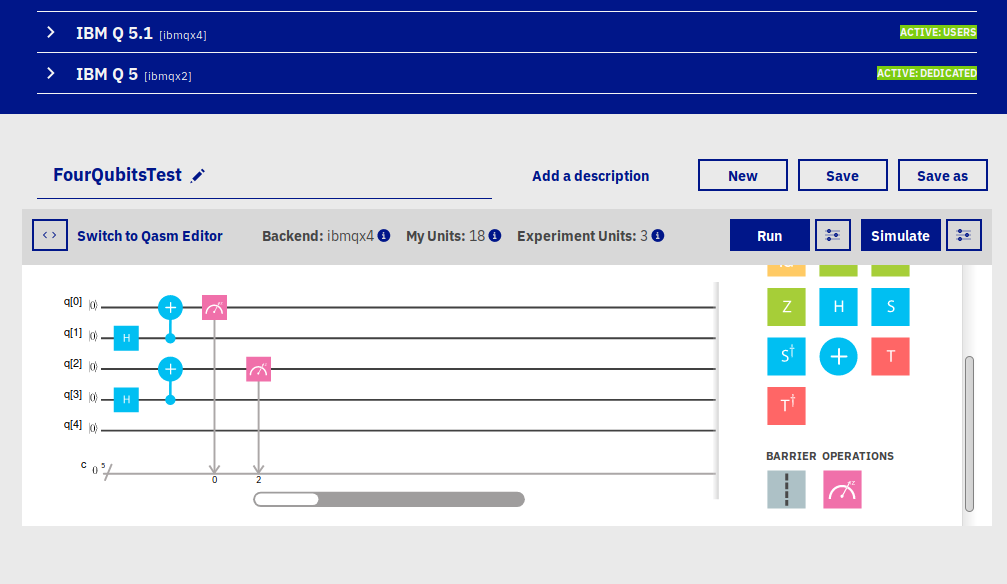
\includegraphics[width=\textwidth]{../slides/pics/ibm-q-experience-composer.png}
\caption{\url{https://quantumexperience.ng.bluemix.net/qx/editor}}
\end{figure}

\begin{figure}[ht!]
\centering
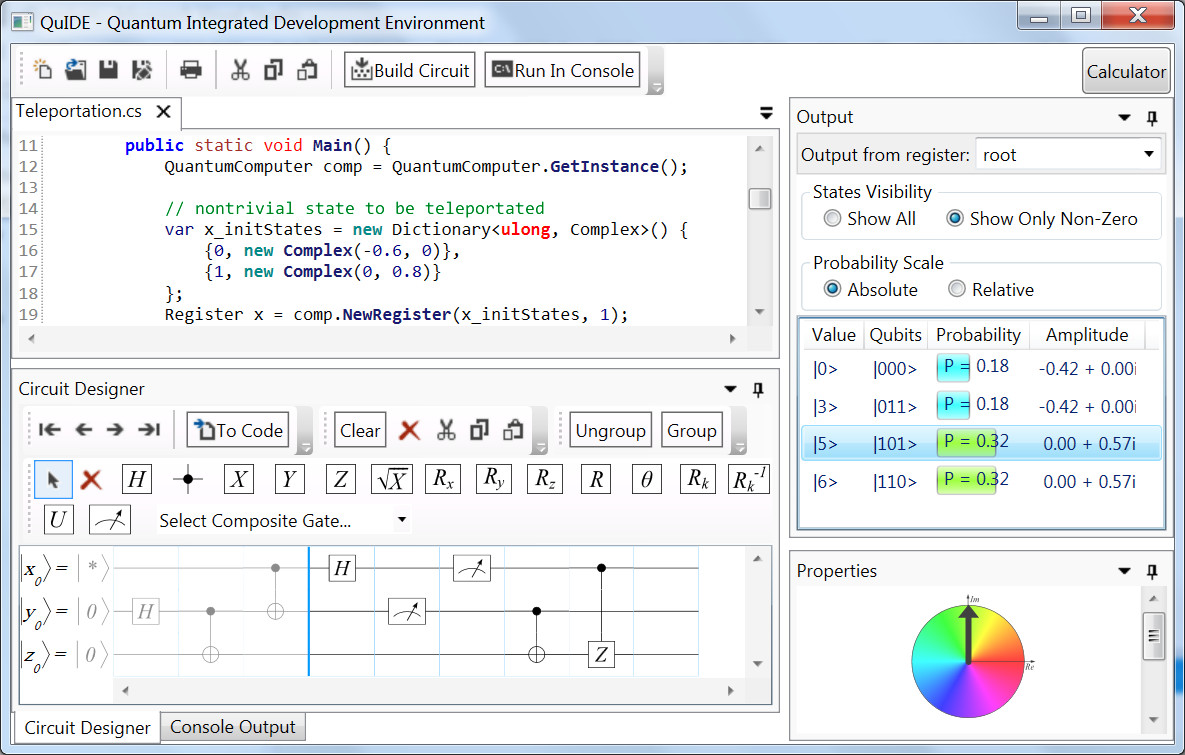
\includegraphics[width=\textwidth]{../slides/pics/QuIDE_GUI.jpg}
\caption{\url{http://www.quide.eu/} and 
\url{https://bitbucket.org/quide/}}
\end{figure}
     



\begin{itemize}
\item Direct manipulation of quantum gates, measurement.
\item Integration with text-based description of circuits: QASM 
(IBM Q) or C\texttt{\#} (QuIDE).
\item Useful for testing small circuits.
\item Not so much for real algorithms.
\item You have to live with connectivity limitations (IBM Q).
\item But you can use a real quantum computer!
\end{itemize}


%%%%%%%%%%%%%%%%%%%%%%%%%%%%%%%%%%%%%%%%%%%%%%%%%%%%%%%%%%%%%%%%%%%%%%%%%%%%%%%%
\subsection{Alternative approach: Manipulation of vectors and matrices}
%%%%%%%%%%%%%%%%%%%%%%%%%%%%%%%%%%%%%%%%%%%%%%%%%%%%%%%%%%%%%%%%%%%%%%%%%%%%%%%%

You already know that
\begin{itemize}
    \item quantum states are just vectors (at least we would like them 
    to 
    be)
    \item ...quantum gates are just matrices (at most $4\times 4$, and 
    don't mention the decoherence)...
    \item ...only the final step is somehow strange.
    \item{\emph{Real Programmers do Quantum Computing in FORTRAN.}}
\end{itemize}


For example, in Julia... \\[12pt] 


\todo{Include Julia code}

\todo{Examples in Wolfram can be found in the GitHub repo}


\begin{itemize}
\item Actually this is almost as good as it gets!
\item Because...
\begin{itemize}
\item ...you already know the language.
\item ...it is very easy to implement 
classical control.
\item ...it is relatively easy to take into account effects of 
decoherence.
\end{itemize}
\item Missing: the memory management.
\item And in most cases you don't need all the power/libraries/etc 
coming with the host language.
\end{itemize}


%%%%%%%%%%%%%%%%%%%%%%%%%%%%%%%%%%%%%%%%%%%%%%%%%%%%%%%%%%%%%%%%%%%%%%%%%%%%%%%%
\subsection{Where to go next?}
%%%%%%%%%%%%%%%%%%%%%%%%%%%%%%%%%%%%%%%%%%%%%%%%%%%%%%%%%%%%%%%%%%%%%%%%%%%%%%%%

\begin{itemize}
\item IBM Q Experience: 
{\small\url{https://quantumexperience.ng.bluemix.net/qx/editor}}
\item Packages/matrix manipulation libraries:
\begin{itemize}
\item quantum-octave (Octave/Matlab): 
{\small \url{https://github.com/ZKSI/quantum-octave}}
\item QuTiP (Python library): {\small\url{http://qutip.org/}}
\end{itemize}
\item Many more at Quantiki 
\url{https://quantiki.org/wiki/list-qc-simulators}
\end{itemize}



%%%%%%%%%%%%%%%%%%%%%%%%%%%%%%%%%%%%%%%%%%%%%%%%%%%%%%%%%%%%%%%%%%%%%%%%%%%%%%
\section{Programming QRAM}
%%%%%%%%%%%%%%%%%%%%%%%%%%%%%%%%%%%%%%%%%%%%%%%%%%%%%%%%%%%%%%%%%%%%%%%%%%%%%%





%%%%%%%%%%%%%%%%%%%%%%%%%%%%%%%%%%%%%%%%%%%%%%%%%%%%%%%%%%%%%%%%%%%%%%%%%%%%%%
\subsection{What is QRAM?}
%%%%%%%%%%%%%%%%%%%%%%%%%%%%%%%%%%%%%%%%%%%%%%%%%%%%%%%%%%%%%%%%%%%%%%%%%%%%%%

\begin{center}
QRAM $\equiv$ Quantum Random Access Machine\\[12pt]
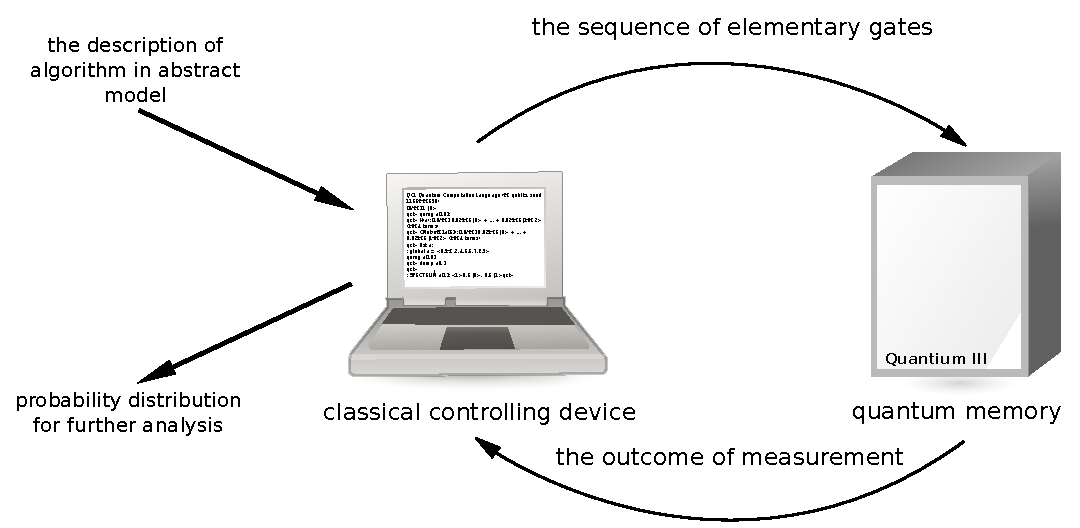
\includegraphics[width=\textwidth]{../slides/pics/qram}
\end{center}


%%%%%%%%%%%%%%%%%%%%%%%%%%%%%%%%%%%%%%%%%%%%%%%%%%%%%%%%%%%%%%%%%%%%%%%%%%%%%%
\subsection{Advantages of QRAM}
%%%%%%%%%%%%%%%%%%%%%%%%%%%%%%%%%%%%%%%%%%%%%%%%%%%%%%%%%%%%%%%%%%%%%%%%%%%%%%

\begin{itemize}
\item data abstraction {$\equiv$ allocation of quantum memory}
\item compound quantum operations <1-3>{\phantom{$\equiv$ 
    functions encapsulating sequence of quantum gates or quantum primitives}}%
{$\equiv$ functions encapsulating sequence of quantum gates or 
quantum primitives}
\item classical control of quantum operations
<1-5>{\phantom{$\equiv$ loops, ifs etc. mixed with quantum code}}%
{$\equiv$ loops, ifs etc. mixed with quantum code}
\end{itemize}



%%%%%%%%%%%%%%%%%%%%%%%%%%%%%%%%%%%%%%%%%%%%%%%%%%%%%%%%%%%%%%%%%%%%%%%%%%%%%%
\subsection{Software architecture}
%%%%%%%%%%%%%%%%%%%%%%%%%%%%%%%%%%%%%%%%%%%%%%%%%%%%%%%%%%%%%%%%%%%%%%%%%%%%%%
%%%%%%%%%%%%%%%%%%%%%%%%%%%%%%%%%%%%%%%%%%%%%%%%%%%%%%%%%%%%%%%%%%%%%%%%%%%%%%


\begin{center}
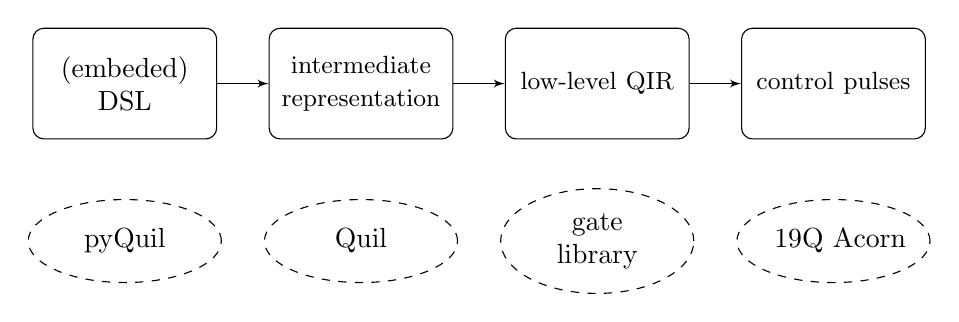
\begin{tikzpicture}[node distance = 3cm, auto]
\tikzstyle{block} = [rectangle, draw, text width=2.1cm, text centered, rounded 
corners, minimum height=4em]
\tikzstyle{example} = [draw, ellipse, node distance=2cm,  text width=1.5cm, 
dashed,
text centered, minimum  height=3em]
\tikzstyle{line} = [draw, -latex', thin]

\node [block] (edsl) {(embeded) DSL};
\node [example, below of=edsl] (edsl-ex) {pyQuil};

\node [block, right of=edsl] (qir) {\small intermediate representation};
\node [example, below of=qir] (qir-ex) {Quil};

\node [block, right of=qir] (qoptim) {\small low-level QIR};
\node [example, below of=qoptim] (qoptim-ex) {gate library};

\node [block, right of=qoptim] (qcontrol) {\small control pulses};
\node [example, below of=qcontrol] (qcontrol-ex) {19Q~Acorn};

\path [line] (edsl) -- (qir);
\path [line] (qir) -- (qoptim);
\path [line] (qoptim) -- (qcontrol);
\end{tikzpicture}
\end{center}



%%%%%%%%%%%%%%%%%%%%%%%%%%%%%%%%%%%%%%%%%%%%%%%%%%%%%%%%%%%%%%%%%%%%%%%%%%%%%%
\subsection{Quantum middleware}
%%%%%%%%%%%%%%%%%%%%%%%%%%%%%%%%%%%%%%%%%%%%%%%%%%%%%%%%%%%%%%%%%%%%%%%%%%%%%%


\begin{itemize}
\item embedded domain specific language $\rightarrow$ 
C/Python/Wolfram/Haskell
with library of functions
\item data abstraction $\rightarrow$ allocation of classical and quantum 
registers based on qu(b$|$d)its
\item quantum functions $\rightarrow$ custom elementary gates defined by 
matrices or compound statements
\item classical control of quantum memory $\rightarrow$ by using host 
language
\end{itemize}


%%%%%%%%%%%%%%%%%%%%%%%%%%%%%%%%%%%%%%%%%%%%%%%%%%%%%%%%%%%%%%%%%%%%%%%%%%%%%%
\subsection{...its advantages...}
%%%%%%%%%%%%%%%%%%%%%%%%%%%%%%%%%%%%%%%%%%%%%%%%%%%%%%%%%%%%%%%%%%%%%%%%%%%%%%

\begin{itemize}
\item easy to learn and use <article>{because you already know 
the language}
\item auto-magic quantum memory management <article>{because 
qubits are just arrays}
\item integration with classical machine
<article>{obviously}
\end{itemize}


%%%%%%%%%%%%%%%%%%%%%%%%%%%%%%%%%%%%%%%%%%%%%%%%%%%%%%%%%%%%%%%%%%%%%%%%%%%%%%
\subsection{...and its disadvantages}
%%%%%%%%%%%%%%%%%%%%%%%%%%%%%%%%%%%%%%%%%%%%%%%%%%%%%%%%%%%%%%%%%%%%%%%%%%%%%%

\begin{itemize}
\item very similar to low-level code <article<>{(but library 
of gates can be build)}
\item lack of expressibility <article>{$\equiv$ you operate on 
basic ingredients only}
\end{itemize}


%%%%%%%%%%%%%%%%%%%%%%%%%%%%%%%%%%%%%%%%%%%%%%%%%%%%%%%%%%%%%%%%%%%%%%%%%%%%%%
\subsection{Example 1: ProjectQ}
%%%%%%%%%%%%%%%%%%%%%%%%%%%%%%%%%%%%%%%%%%%%%%%%%%%%%%%%%%%%%%%%%%%%%%%%%%%%%%


\begin{itemize}
\item Python library developed by ETH (\url{https://projectq.ch/})
\item offers various targets
\begin{itemize}
\item hardware (IBM Q Experience) 
<article>{(\verb|use_hardware=False|)}
\item resource counter (???)
\item graphical circuit representation
\end{itemize}
\end{itemize}



%%%%%%%%%%%%%%%%%%%%%%%%%%%%%%%%%%%%%%%%%%%%%%%%%%%%%%%%%%%%%%%%%%%%%%%%%%%%%%

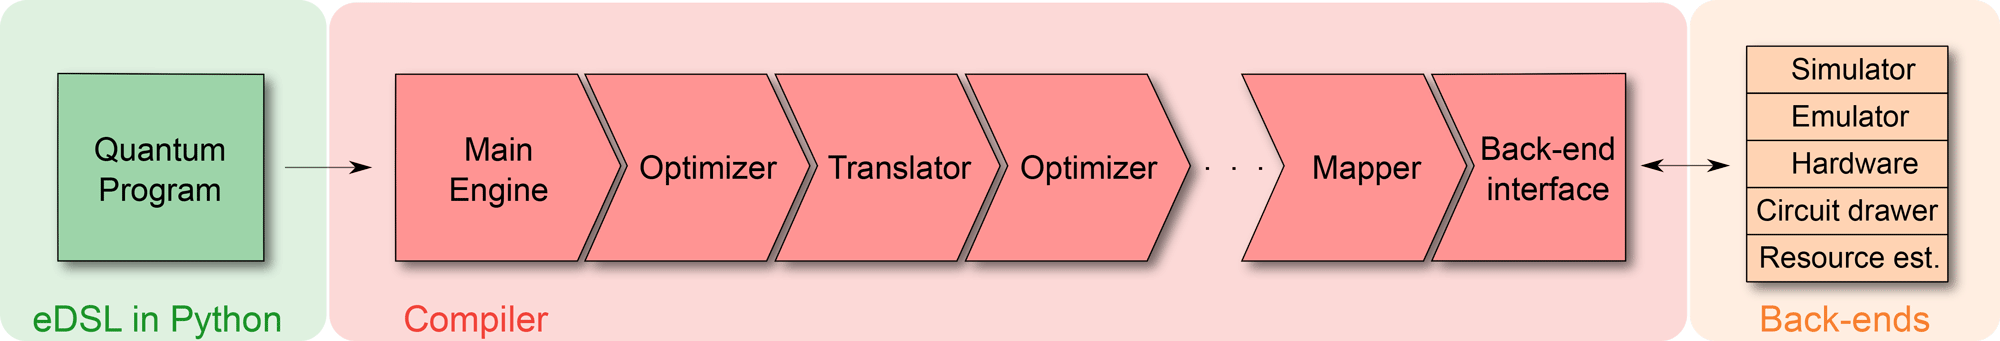
\includegraphics[width=\textwidth]{../slides/pics/projectq-compiler-overview.png}\\



%%%%%%%%%%%%%%%%%%%%%%%%%%%%%%%%%%%%%%%%%%%%%%%%%%%%%%%%%%%%%%%%%%%%%%%%%%%%%%

Nice features
\begin{itemize}
\item Natural (for physicist) syntax for executing quantum gates.
\item Meta instructions for quantum-controlled quantum operations and 
support for reverse call
<article>{(very easy to construct controlled operations)}
\end{itemize}


%%%%%%%%%%%%%%%%%%%%%%%%%%%%%%%%%%%%%%%%%%%%%%%%%%%%%%%%%%%%%%%%%%%%%%%%%%%%%%

Some examples...


%%%%%%%%%%%%%%%%%%%%%%%%%%%%%%%%%%%%%%%%%%%%%%%%%%%%%%%%%%%%%%%%%%%%%%%%%%%%%%

{Metainstruction \texttt{Control}}
Execution of the code is based on the state of quantum register.


\begin{center}
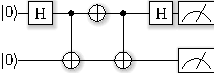
\includegraphics[scale=1.5]{../slides/pics/meta_control_circ.pdf}
\end{center}


%%%%%%%%%%%%%%%%%%%%%%%%%%%%%%%%%%%%%%%%%%%%%%%%%%%%%%%%%%%%%%%%%%%%%%%%%%%%%%

{Metainstruction \texttt{Dagger}}
Reverse execution of the quantum code.


\begin{center}
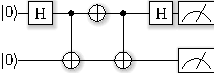
\includegraphics[scale=1.5]{../slides/pics/meta_dagger_circ.pdf}
\end{center}


%%%%%%%%%%%%%%%%%%%%%%%%%%%%%%%%%%%%%%%%%%%%%%%%%%%%%%%%%%%%%%%%%%%%%%%%%%%%%%
\subsection{Example 2: Rigetti Forest and pyQuil}
%%%%%%%%%%%%%%%%%%%%%%%%%%%%%%%%%%%%%%%%%%%%%%%%%%%%%%%%%%%%%%%%%%%%%%%%%%%%%%


\begin{itemize}
\item Quil $\equiv$ quantum assembly language.
\item pyQuil $\equiv$ Python library for manipulating quantum 
programmes in Quill.
\item Access to Rigetti 19Q-Acorn quantum computer!
\item More during the third day: Adam Szady, Quantum programming 
with (Py)Quil.
\end{itemize}



%%%%%%%%%%%%%%%%%%%%%%%%%%%%%%%%%%%%%%%%%%%%%%%%%%%%%%%%%%%%%%%%%%%%%%%%%%%%%%
\section{High-level programming}
%%%%%%%%%%%%%%%%%%%%%%%%%%%%%%%%%%%%%%%%%%%%%%%%%%%%%%%%%%%%%%%%%%%%%%%%%%%%%%


%%%%%%%%%%%%%%%%%%%%%%%%%%%%%%%%%%%%%%%%%%%%%%%%%%%%%%%%%%%%%%%%%%%%%%%%%%%%%%
\subsection{Domain specific languages}
%%%%%%%%%%%%%%%%%%%%%%%%%%%%%%%%%%%%%%%%%%%%%%%%%%%%%%%%%%%%%%%%%%%%%%%%%%%%%%



{Level 2}
Domain specific language with data and function abstraction.


\begin{itemize}
\item QCL (\url{http://tph.tuwien.ac.at/~oemer/qcl.html})
\item LanQ (\url{http://lanq.sourceforge.net/})
\item QPL anc cQPL (\url{https://arxiv.org/abs/quant-ph/0511145})
\item Scaffold (\url{https://github.com/epiqc/ScaffCC})
\end{itemize}



%%%%%%%%%%%%%%%%%%%%%%%%%%%%%%%%%%%%%%%%%%%%%%%%%%%%%%%%%%%%%%%%%%%%%%%%%%%%%%
\subsection{Example 1: QCL -- focus on quantum computing}
%%%%%%%%%%%%%%%%%%%%%%%%%%%%%%%%%%%%%%%%%%%%%%%%%%%%%%%%%%%%%%%%%%%%%%%%%%%%%%

%%%%%%%%%%%%%%%%%%%%%%%%%%%%%%%%%%%%%%%%%%%%%%%%%%%%%%%%%%%%%%%%%%%%%%%%%%%%%%

\begin{itemize}
\item First release in 1998, last in 2014 
(\url{http://tph.tuwien.ac.at/~oemer/qcl.html}).
\item Architecture independent programming language for quantum 
computers.

\end{itemize}



%%%%%%%%%%%%%%%%%%%%%%%%%%%%%%%%%%%%%%%%%%%%%%%%%%%%%%%%%%%%%%%%%%%%%%%%%%%%%%

Features
\begin{itemize}
\item Syntax for reversibility (uncomputing).
\item Different types of quantum memory for better optimization.
\item Quantum conditions --- quantum-controlled execution 
(generalization of controlled 
gates).
\item Various types of compound statements (related with memory 
management): quantum operators, quantum functions, procedures.

\end{itemize}


%%%%%%%%%%%%%%%%%%%%%%%%%%%%%%%%%%%%%%%%%%%%%%%%%%%%%%%%%%%%%%%%%%%%%%%%%%%%%%

Advanced quantum memory management using types:
\begin{itemize}
\item \texttt{qureg} ---  basic type for quantum registers,
\item \texttt{quconst} --- cannot be modified,
\item \texttt{quvoid} --- has to be empty before the call,
\item \texttt{quscratch} --- has to be empty before and after the 
call.
\end{itemize}

Types of quantum functions:
\begin{itemize}
\item \texttt{procedure} ---  classically controlled quantum 
computation,
\item \texttt{qufunct} --- used to implement irreversible functions,
\item \texttt{operator} --- compound quantum operation.
\end{itemize}


%%%%%%%%%%%%%%%%%%%%%%%%%%%%%%%%%%%%%%%%%%%%%%%%%%%%%%%%%%%%%%%%%%%%%%%%%%%%%%

Some examples...


%%%%%%%%%%%%%%%%%%%%%%%%%%%%%%%%%%%%%%%%%%%%%%%%%%%%%%%%%%%%%%%%%%%%%%%%%%%%%%
\subsection{Example 2: cQPL -- focus on quantum communication}
%%%%%%%%%%%%%%%%%%%%%%%%%%%%%%%%%%%%%%%%%%%%%%%%%%%%%%%%%%%%%%%%%%%%%%%%%%%%%%

%%%%%%%%%%%%%%%%%%%%%%%%%%%%%%%%%%%%%%%%%%%%%%%%%%%%%%%%%%%%%%%%%%%%%%%%%%%%%%


\begin{itemize}
\item QPL (formal specification) and cQPL (implementation of QPL, 
\url{https://arxiv.org/abs/quant-ph/0511145})
\item Functional paradigm.
\item No publicly available implementation.
\item Syntax for creating quantum communication channels by sharing 
(entangled) qubits.
\end{itemize}


%%%%%%%%%%%%%%%%%%%%%%%%%%%%%%%%%%%%%%%%%%%%%%%%%%%%%%%%%%%%%%%%%%%%%%%%%%%%%%%
%\section{What next?}
%%%%%%%%%%%%%%%%%%%%%%%%%%%%%%%%%%%%%%%%%%%%%%%%%%%%%%%%%%%%%%%%%%%%%%%%%%%%%%%
%
%%%%%%%%%%%%%%%%%%%%%%%%%%%%%%%%%%%%%%%%%%%%%%%%%%%%%%%%%%%%%%%%%%%%%%%%%%%%%%%
%
%\begin{itemize}
%\item \textbf{IF} D-Wave \textbf{GOTO} Andy Mason and Sheir Yarkoni, 
%Tutorial on 
%programming the D-Wave system
%\item \textbf{IF} IBM \textbf{GOTO} Ram Du\v{s}i\'c Hren, IBM Q 
%Experience: Hands-on workshop
%\item \textbf{IF} Rigetti \textbf{GOTO} Adam Szady, Quantum programming 
%with (Py)Quil
%\end{itemize}

\end{document}
